\providecommand{\CryptoDisk}{<<{Криптодиск}>>\xspace}

\chapter{Общие положения}\label{Common}

\section{Назначение}

Настоящий стандарт устанавливает требования безопасности к программным 
средствам криптографической защиты информации.
ПСКЗИ представляет собой набор программ и связанных с ними данных,
который реализует криптографические алгоритмы и протоколы,
а также дополнительно:
\begin{itemize}
\item[--]
функции управления данными,
включая средства генерации, экспорта, импорта и уничтожения
ключей;

\item[--]
механизмы контроля доступа к данным,
включая средства идентификации и аутентификации;

\item[--]
механизмы проверки работоспособности,
включая средства тестирования, диагностики и 
контроля целостности,
%
предназначенные для безопасного управления вызовами
криптографических алгоритмов и их входными и выходными данными.
\end{itemize}

Требования безопасности делятся на 
функциональные~(разделы~\ref{FReqsTOE}, \ref{FReqsEnv}) 
и гарантийные~(раздел~\ref{AReqs}).
Функциональные требования направлены на решение задач безопасности,
гарантийные требования поддерживают качество решения данных задач.
%
Функциональные требования обеспечивают противодействие угрозам безопасности, 
следование определенным правилам безопасности.
%
Гарантийные требования обеспечивают доверие к тому, 
что программное средство корректно спроектировано и разработано, 
протестировано в достаточном объеме, 
правильно установлено и эксплуатируется.

Программы~\TOE выполняются в определенной среде эксплуатации~---
на персональном компьютере, в мобильном устройстве, на смарт-карте и др.
Среда эксплуатации обеспечивает~\TOE процессорными ресурсами, 
ресурсами памяти, а также предоставляет системные средства 
управления этими ресурсами.
%
Программное средство зависимо от ресурсов среды 
и не в состоянии обеспечить безопасность своих объектов самостоятельно.
Поэтому функциональные требования реализуются
как средствами~\TOE~(раздел~\ref{FReqsTOE}),
так и средствами среды~(раздел~\ref{FReqsEnv}).

Требования безопасности задают разбиение~\TOE
на два класса. К средствам первого класса выдвигается 
базовый набор требований, к средствам второго~--- усиленный.
%
Средства второго класса рекомендуется использовать
в тех случаях, когда возможны изменения критических системных 
компонентов в среде эксплуатации,
например, если разрешена установка новых программ,
обновление операционной системы, 
замена оборудования и др.
%
Средства второго класса рекомендуется применять также тогда,
когда гипотетический нарушитель имеет возможность 
наблюдать за побочными каналами,
например за временем выработки ЭЦП на смарт-карте.
	
Методы реализации требований безопасности 
описываются в функциональной спецификации. 
%
Функциональная спецификация может представлять собой 
отдельный документ либо разделы нескольких документов.
%
Примерное содержание функциональной спецификации представлено 
в приложении~\ref{SPEC}.
%
Приложение~\ref{EXAMPLE} содержит примерную спецификацию гипотетического 
программного средства~\CryptoDisk.

\section{Криптографическая поддержка}

\TOE реализует один или несколько криптографических алгоритмов 
или протоколов. Алгоритмы и протоколы используются 
как в доступных извне сервисах, 
так и во внутренних средствах безопасности, 
обеспечивающих защиту объектов.

Входные данные криптографического алгоритма делятся на служебные и собственно 
обрабатываемые (содержательные) объекты. 
К служебным объектам относятся долговременные параметры, 
которые задают семейство криптографических преобразований для данного алгоритма,
ключи, которые определяют выбор одного преобразования из семейства, 
синхропосылки, которые обеспечивают уникальность результатов 
преобразования на фиксированном ключе, и др.

Криптографические алгоритмы делятся на
алгоритмы с секретным ключом (симметричные),
алгоритмы с открытым ключом (асимметричные) 
и бесключевые алгоритмы.
%
В симметричных алгоритмах для выполнения нескольких связанных
операций, например зашифрования и расшифрования,
используется один и тот же секретный ключ. 
%
В асимметричных алгоритмах используется пара ключей~--- 
личный и соответствующий ему открытый.
Например, в алгоритмах ЭЦП при выработке подписи используется 
личный ключ, а при ее проверке~--- открытый.
%
К бесключевым относятся алгоритмы хэширования, 
алгоритмы разделения секрета, 
алгоритмы построения семейства ключей по одному главному ключу. 
В этих алгоритмах ключи, отвечающие за выбор 
криптографического преобразования,
не используются, хотя обрабатываемые объекты сами могут являться 
ключами~\forref{CryptoAlg}.

При реализации криптографических алгоритмов разрешается 
сужать множество обрабатываемых объектов. 
Например, алгоритм шифрования может обрабатывать сообщения не любой,
а только определенной длины.
Вместе с тем сужение множества ключей не допускается~\forref{CryptoAlg}.

Кроме собственно криптографических алгоритмов, их спецификации могут 
определять методы генерации долговременных параметров и ключей.
Методы могут определяться рамочно, без исчерпывающих деталей.
%
Например, при генерации параметров ЭЦП на основе эллиптических кривых 
используются вспомогательные алгоритмы проверки простоты чисел, 
расчета порядка группы точек эллиптической кривой, 
извлечения квадратных корней и др., 
которые могут быть не определены в спецификации.
%
При реализации в~\TOE методов генерации параметров проводится 
уточнение вспомогательных алгоритмов.
%
Уточнения могут касаться также способов генерации случайных чисел,
по которым строятся искомые долговременные параметры или ключи~\forref{CryptoGen}.

Криптографические протоколы представляют собой наборы 
криптографических алгоритмов, которые выполняются в определенной
последовательности двумя (или более) сторонами. 
Для протоколов также справедливы приведенные выше пояснения.

В~\TOE реализуются средства тестирования криптографических алгоритмов 
и протоколов. Для тестирования могут использоваться:
тесты известного ответа, тесты прямого и обратного преобразований, 
тесты на соответствие между открытым и личным ключами~\forref{SelfTests}.

\section{Операторы}

С~\TOE взаимодействуют операторы.
%
Взаимодействие состоит в работе с сервисами.
%
При использовании сервиса оператор 
готовит и передает входные данные и управляющие параметры сервиса,
вызывает сервис, получает и обрабатывает выходные данные.

Некоторые операции могут выполняться не одним, а несколькими сервисами. 
Например, защита канала связи может быть реализована сервисом 
выработки общего сеансового ключа и сервисом шифрования данных канала.
Определенные последовательности вызовов сервисов могут быть запрещены. 
Например, запрещено выполнять шифрование до выработки 
общего сеансового ключа~\forref{Services}.

Сервисы доступны операторам через устройства ввода/вывода 
(клавиатуру, дисплей, принтер, порты) и логические интерфейсы
(например, наборы функций динамических библиотек).
%
Оператор может взаимодействовать с~\TOE не напрямую, 
а через клиентские программы (клиентов электронной почты, браузеры, 
программы управления электронными документами). 
%Клиентские программы выступают от лица операторов и отождествляются с ними.

\TOE поддерживает определенные роли (категории) операторов.
Имеется роль <<Администраторы>>.
Операторы этой роли наделены правами выполнять 
административные сервисы~\TOE:
устанавливать и настраивать~\TOE, 
управлять правами операторов, вводить мастер-ключи.
%
Рекомендуется определять роль <<Пользователи>>.
Пользователи выполняют общие сервисы \TOE:
шифруют почтовые отправления, проверяют ЭЦП электронных документов,
генерируют ключи~\forref{DAC}.

Имеется предопределенная роль <<Система>>,
которая явно может не определяться.
Неявный оператор этой роли (системный оператор)
выполняет внутренние сервисы~\TOE:
самотестирование при загрузке, 
контроль доступа, управление состояниями сеансов.

%Могут вводиться дополнительные роли.
Один и тот же оператор может выполнять сразу несколько 
ролей~\forref{Identification}.

\section{Аутентификация}

В~среде эксплуатации~\TOE реализуются средства аутентификации 
для проверки принадлежности оператора к явным ролям 
и допустимости выполнения оператором 
сервисов данных ролей. 
%
Аутентификация требуется также для проверки прав доступа вызываемых 
оператором сервисов к открытым и критическим объектам. 
Полный доступ к таким объектам разрешается, как правило,
только владельцам и для проверки полномочности доступа кроме 
роли, используется также идентификатор оператора.
%
Допускается, что для выполнения некоторых сервисов 
или доступа к некоторым 
объектам требуется дополнительная аутентификация~\forref{Authentication}.

Средства аутентификации могут быть полностью или частично реализованы 
самим~\TOE.

Методы аутентификации
основываются на использовании комбинаций из трех факторов: 
владение операторами устройствами аутентификации (<<что я имею>>), 
знание секретов аутентификации (<<что я знаю>>), 
обладание биометрическими характеристиками (<<кто я>>).
Рекомендуется задействовать более одного фактора, например использовать 
карты доступа вместе с PIN-кодами доступа~\forref{Auth2Factor}.

При аутентификации операторы предъявляют
устройства аутентификации (смарт-карты) 
и вводят аутентификационные данные (пароли, отпечатки пальцев).
%
Средства аутентификации проверяют корректность представленных устройств и 
сравнивают характеристики аутентификационных данных 
с контрольными значениями.

При создании и изменении секретов аутентификации предусматривается 
проверка их качества. Проверка может состоять в контроле 
длины пароля или контроле включения в пароль как цифровых, 
так и буквенных символов в различных регистрах.
Проверка качества секретов не может основываться на ограничениях 
в руководствах, \ie на предположении о том, что оператор
обязательно задаст пароль нужного качества~\forref{PwdSet}.

\section{Сеансы}

Взаимодействие оператора с~\TOE происходит в форме сеансов. 
В начале сеанса, как правило, 
выполняются сервисы идентификации и аутентификации оператора,
в конце сеанса~--- очистка и уничтожение сеансовых объектов.
%
Отдельно выделяется системный сеанс неявного системного оператора,
который совпадает с непрерывным периодом работы~\TOE
(от загрузки до выгрузки программ). 

Системный сеанс~\TOE может находиться в одном из нескольких состояний,
которые характеризуются различными правами доступа к сервисам. 
%
Имеются состояния, соответствующие сеансам операторов различных ролей. 
В этих состояниях операторы могут выполнять сервисы в соответствии 
с политикой управления доступом. 
%
Имеется также состояние блокировки,
в котором выполнение сервисов запрещается или сильно ограничивается.
%
Примеры других состояний системного сеанса:
<<самотестирование>>,
<<ожидание>> (до аутентификации операторов),
<<временная блокировка>> (блокировка на определенный период времени
после превышения порога неудачных попыток аутентификации) и др.
%
Могут определяться подчиненные состояния,
например внутренние состояния сеансов администратора и пользователя~\forref{States}.

Блокировка может состоять в принудительном завершении программ~\forref{LockState}.

Многозадачные операционные системы могут поддерживать 
одновременное выполнение сеансов для нескольких операторов~\TOE.
При этом состояния <<сеанс администратора>>, 
<<сеанс пользователя>> могут дублироваться. 
Считается, что~\TOE одновременно может находиться
сразу во всех состояниях, соответствующих сеансам операторов. 
Такой режим реализуется средствами обеспечения 
многозадачности операционной системы~\forref{States}.

%Один из возможных способов организации такой 
%поддержки состоит в следующем (рисунок~\ref{Fig.Descr.Session}).
%Клиентская программа является отдельным процессом операционной системы 
%с~защищенным от других процессов адресным пространством.
%Сеансами являются отдельные потоки клиентского процесса. 
%Данные сеансов одного процесса не защищены друг от друга,
%но защищены от данных сеансов других процессов.
%Для одновременного доступа к одним и тем же объектам
%нескольких сеансов средствами~\TOE или операционной системы 
%реализуются механизмы синхронизации.

\section{Объекты}

С помощью сервисов операторы выполняют операции над объектами~---
ключами, открытыми текстами, параметрами криптографических алгоритмов,
сертификатами открытых ключей и др.

Объекты делятся на открытые (общедоступные) 
и критические (ограниченного доступа).
%
Например, открытый ключ подписи является открытым объектом,
личный ключ подписи~--- критическим~\forref{Objects}.

Кроме этого, объекты делятся на сеансовые и долговременные.
Сеансовые объекты создаются во время сеансов операторов и уничтожаются
при их завершении. 
Доступ к таким объектам имеет только оператор сеанса.
Долговременные объекты существуют как во время, 
так и вне времени выполнения сеансов, 
хранятся в пределах криптографической границы
или передаются за ее пределы.
Доступ к долговременным объектам имеют все операторы 
с соответствующими правами.
Например, личный ключ подписи на магнитном носителе является 
долговременным объектом, а генерируемое при выработке подписи 
случайное число~--- сеансовым~\forref{Objects}.

У объектов есть владельцы.
Например, объектами администратора 
являются журнал аудита (критический объект),
настройки политики управления доступом (открытый объект).
%
Пользователи владеют идентификаторами, ключами, документами.
Файлы программ и конфигураций относятся к системным объектам,
владельцем которых является неявный системный оператор~\forref{Objects}.

При выполнении сервисов~\TOE может создаваться несколько
сеансовых копий одного и того же объекта 
в нескольких переменных программ. 
Сеансовые копии не обязательно определять как отдельные объекты,
достаточно обеспечить очистку сеансовых копий 
критических объектов~\forref{Objects}.
%и защиту от создания неявных копий критических объектов~\forref{Objects}.
%\footnote{сеансовые копии vs неявные копии -- не очень понятно}

К объектам~\TOE не относятся секреты аутентификации. 
При передаче таких секретов от операторов 
сервисам их защита обеспечивается средствами среды эксплуатации. 
Однако контрольные значения секретов являются долговременными объектами~\TOE. 
Кроме этого, в ходе сеансов на основе аутентификационных данных могут 
вырабатываться сеансовые объекты (например, хэш-значение пароля, 
используемое в качестве ключа), которые защищаются 
средствами~\TOE~\forref{Objects}.

%\begin{figure}[bht]
%\begin{center}
%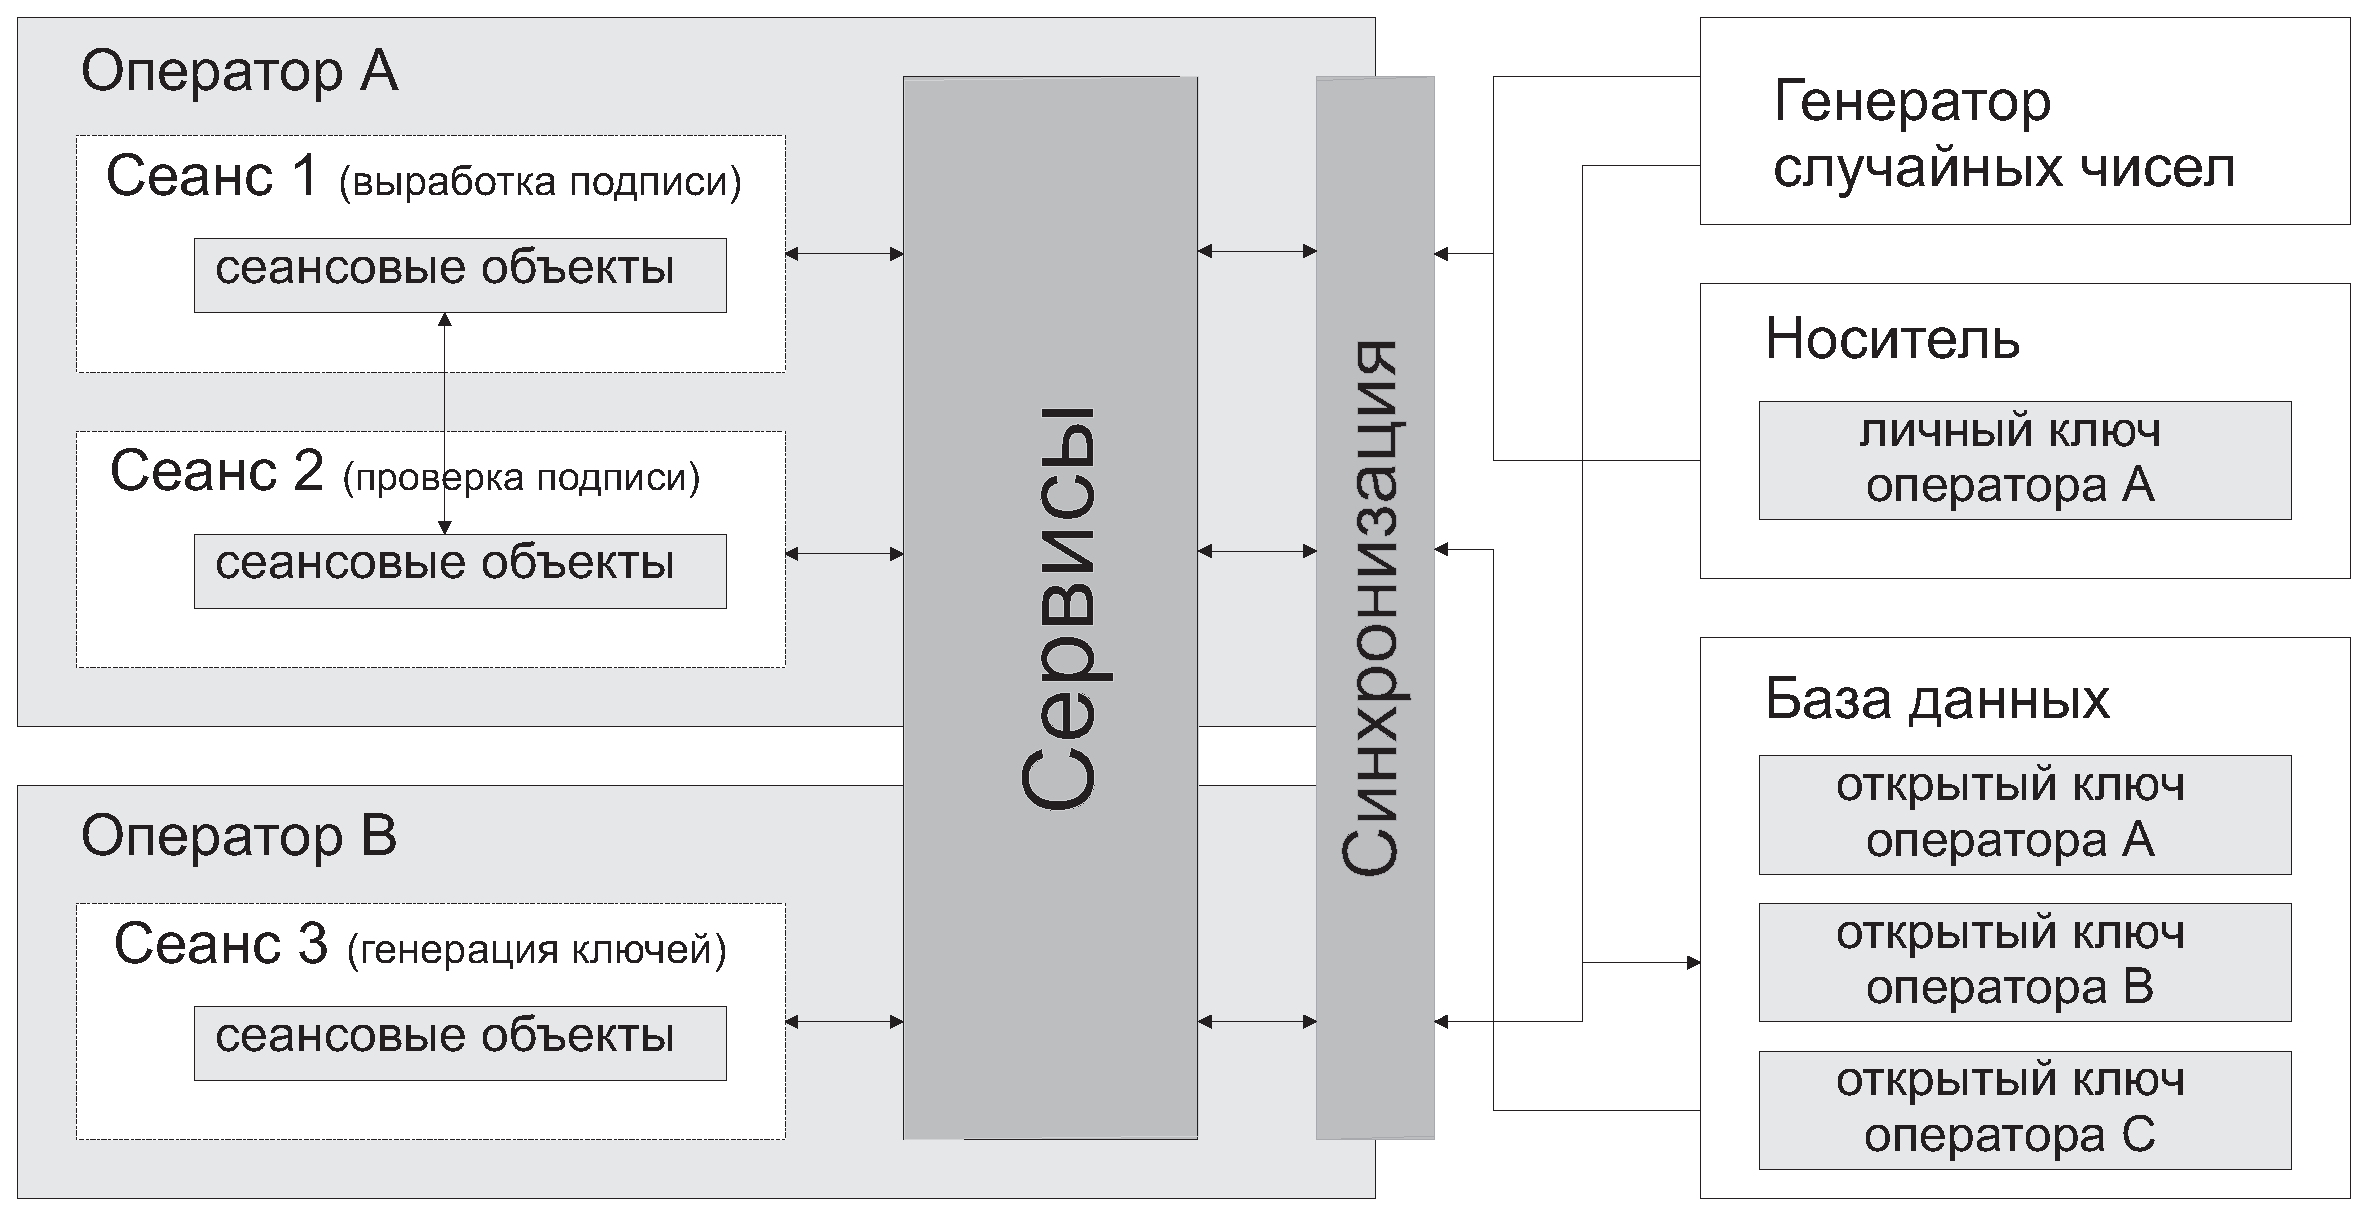
\epsfig{file=Session.eps,width=13cm}
%\end{center}
%\caption{Сеансы и объекты}\label{Fig.Descr.Session}
%\end{figure}

Обращения операторов, прошедших аутентификацию, к сервисам и объектам~\TOE 
регулируются политикой управления доступом. 
Политика регламентирует набор допустимых 
операций операторов над сервисами и объектами.
%
Список разрешенных операций определяется идентификатором и ролью 
оператора, типом объекта, владельцем объекта, 
состоянием, в котором находится сеанс оператора, и другими условиями.
%
Список операций может включать: 
выполнение сервисов,
создание,
удаление,
экспорт,
импорт,
чтение, 
запись объектов~\forref{DAC}.

\section{Защита объектов}

Сеансовый объект может быть преобразован в долговременный,
\ie может экспортироваться за пределы сеанса.
%
При экспорте сеансовые объекты защищаются, \ie обеспечивается
\begin{itemize}
\item[--]
конфиденциальность критических объектов;
\item[--]
контроль целостности открытых и критических объектов.
\end{itemize}

%Экспортом не считается передача объекта во владение другому сеансу доверенного
%СКЗИ в криптографической границе. 
%%
%Рассмотрим пример. Пусть в некотором ПСКЗИ 
%реализован сервис генерации случайных чисел.
%Сервис вызывает другое ПСКЗИ и использует 
%случайные числа для создания ключа, 
%который затем сохраняется на смарт-карте.
%%
%Случайные числа являются критическим сеансовым объектом первого средства
%и передаются во владение второму. 
%Личный ключ является критическим сеансовым объектом второго средства
%и экспортируется на смарт-карту.

%
%Защита критических объектов выполняется непосредственно
%при экспорте средствами~\TOE.
%%
%Защита открытых объектов и частичных секретов 
%выполняется либо непосредственно 
%при экспорте средствами~\TOE, либо позже средствами доверенных~СКЗИ.
%%
%В последнем случае ответственность за отложенную защиту возлагается
%на среду экcплуатации.

Обратно долговременные объекты могут импортироваться из-за 
пределов сеанса. При импорте проверяется целостность 
объектов и дополнительно критические объекты преобразуются 
из защищенной формы в открытую, например расшифровываются.

Для защиты объектов используются следующие методы:

1~{\it Криптографические методы}. 
Состоят в применении алгоритмов шифрования 
(блочного, поточного, с открытым ключом)
для обеспечения конфиденциальности,
алгоритмов ЭЦП и имитозащиты для контроля 
целостности~\forref{DPTCryptoEncr},
\forref{DPTCryptoIntegrity}.

2~{\it Аппаратные методы}. 
Состоят в аппаратной защите от несанкционированного
чтения и (или) модификации областей памяти,
в которых размещаются целевые объекты.
Аппаратная защита обеспечивается применением смарт-карт, токенов
и других подобных устройств~\forref{DPTHard}. 

%Tamper-Resistant Security Module (TRSM) must
%meet the requirements of a Physically Secure Device
%as defined in ISO 9564-1. Such a device must have a
%negligible probability of being successfully penetrated
%to disclose all or part of any secret or private
%cryptographic key or PIN. A TRSM can be so certified
%only after it has been determined that the device’s
%internal operation has not been modified to allow
%penetration (e.g., the insertion within the device of an
%active or passive “tapping” mechanism).

3~{\it Методы разделения секрета}. 
Состоят в разбиении защищаемого критического объекта на частичные секреты, 
каждый из которых затем защищается по отдельности.
%
Простейшим методом разделения секрета является представление
ключа как двоичного слова в виде суммы (поразрядной по модулю $2$)
нескольких частичных секретов. 
В этом случае для восстановления исходного 
ключа требуется располагать всеми частичными секретами.
%
Более сложные пороговые методы позволяют 
определить исходный ключ при наличии не всех, 
а только порогового числа частичных секретов, 
например трех из пяти~\forref{DPTSplit}.

4~{\it Алгоритмические методы}. 
Состоят в контроле целостности с помощью некриптографических или 
бесключевых криптографических алгоритмов.
К алгоритмическим методам относятся: 
сверка нескольких копий объекта, 
проверка контрольных хэш-значений,
самоподпись сертификата открытого ключа~\forref{DPTAlgo}.

5~{\it Организационные меры}. 
Состоят в обеспечении конфиденциальности с помощью мероприятий,
не относящихся к информационным технологиям.

При выборе методов защиты предпочтение следует отдавать 
криптографическим методам. Однако для организации криптографической защиты 
объектов при экспорте и импорте требуется использовать другие 
объекты-ключи. Если эти объекты также нужно экспортировать или 
импортировать, то для их защиты должны использоваться новые ключи
и т.~д. Аппаратные методы и методы разделения секрета позволяют
прервать цепочку ключей защиты других ключей.

В алгоритмических методах защиты контрольная характеристика, 
на основании которой принимается решение о целостности объекта, 
может не защищаться и храниться вместе с самим объектом.
Тогда алгоритмический метод обеспечивает защиту только от случайных сбоев 
в среде эксплуатации, но не от преднамеренного воздействия. 
%
Если же контрольная характеристика защищается, то защита распространяется
на контролируемый объект. 
%
Пусть, например, \TOE вырабатывает личный и открытый ключи,
сохраняет личный ключ на смарт-карту, 
а открытый ключ отсылает в удостоверяющий центр для получения сертификата. 
%
После получения сертификата \TOE вычисляет по сохраненному личному ключу 
открытый и сравнивает его с ключом, размещенным в сертификате.
%
Проверка связи между ключами соответствует алгоритмическому методу защиты.
Аппаратная защита личного ключа распространяется в момент импорта
на открытый ключ сертификата. 

Защита критических сеансовых объектов включает невозможность 
их определения после завершения сеансов.
Для очистки сеансовых объектов в оперативной памяти можно использовать 
обнуление ячеек памяти,
а для очистки объектов в постоянной перепрограммируемой памяти 
может быть использована многократная перезапись ячеек 
константами и случайными данными~\forref{DPTZeroization}.

\section{Среда эксплуатации}

Для учета возможных уязвимостей в среде эксплуатации 
разработчик определяет криптографическую границу~---
непрерывный физический периметр, 
который задает контролируемую границу~\TOE.

В криптографической границе~\TOE выделяются
критические системные компоненты~--- 
аппаратное и программное обеспечение, которое используется
для передачи, обработки и хранения объектов~\TOE.
%(рисунок~\ref{Fig.Descr.TOE}).
К критическим системным компонентам относятся:
\begin{itemize}
\item[--]
устройства ввода/вывода;

\item[--]
устройства обработки и передачи (процессор, физические интерфейсы);

\item[--]
устройства хранения (жесткий диск);

\item[--]
службы операционной системы, влияющие на безопасность~\TOE;

\item[--]
дополнительное оборудование (генераторы случайных чисел).
\end{itemize}

%\begin{figure}[bht]
%\begin{center}
%\epsfig{file=TOE.eps,width=13cm}
%\end{center}
%\caption{\doubt{Среда эксплуатации}}\label{Fig.Descr.TOE}
%\end{figure}

\TOE не может обеспечить безопасность критических системных компонентов,
обеспечение безопасности возлагается на среду.
%
Перед установкой и использованием~\TOE производится настройка среды. 
При настройке конфигурируются средства защиты операционной системы, 
задаются разрешения на установку программ, 
вводятся ограничения на доступ к системным объектам и др.

В~\TOE предусматриваются средства проверки  
условий безопасности среды, 
направленные на контроль состава и правильного 
функционирования критических компонентов.
%
Проверки могут быть косвенными. 
Например, успешная загрузка операционной системы
может являться основанием для вывода о корректности работы
устройств обработки и запоминающих устройств.
В свою очередь проверка
операционной системы может заключаться в контроле версий ее модулей.
%
В большинстве случаев нельзя провести исчерпывающее тестирование 
критических системных компонентов. Допускается, что при тестировании 
проверяется только их наличие и проводится контроль лишь нескольких 
их основных функций.
%
Для некоторых компонентов при начальном запуске можно провести лишь часть 
проверок. В таких случаях разрешается выполнить пропущенные тесты позднее.
Например, при начальном запуске проверяется
наличие устройства чтения смарт-карт, 
а корректность работы данного устройства проверяется 
при непосредственном чтении данных с карты~\forref{CSCTests}.

При обработке объектов~\TOE в критических системных компонентах
могут появляться побочные каналы, по которым передается информация
о критических объектах. 
%
Например, алгоритм выработки ЭЦП может быть реализован таким образом,
что по времени его выполнения нарушитель может сделать вывод 
о значении некоторых битов личного ключа~\forref{CryptoTiming}. 

Побочным каналом является канал сохранения неявных 
копий сеансовых объектов в файле подкачки, регистрах процессора, 
журнале аудита~\forref{LeakProtect}.

В~\TOE второго класса предусматриваются средства защиты от побочных каналов.

\section{Генерация случайных чисел}

В криптографической границе \TOE могут находиться генераторы случайных
чисел, которые вырабатывают данные для создания 
секретных и личных ключей, синхропосылок, других критических или 
уникальных объектов.
К генераторам случайных чисел не относятся 
алгоритмы выработки псевдослучайных чисел,
хотя ключи таких алгоритмов могут строиться с помощью генераторов.

Генератор случайных чисел выдает последовательности,
каждый следующий элемент которых 
статистически и вычислительно трудно предсказать 
по всем предыдущим элементам.
%
Генератор использует один или несколько 
источников случайности (неопределенности, энтропии)
и включает средства обработки данных от источников. 
%
Средства обработки могут частично или полностью 
размещаться в~\TOE~\forref{RNG}.

В компьютерных системах 
используются следующие источники случайности~\forref{RNG}:
\begin{itemize}
\item[--]
физические источники, использующие процессы в физических устройствах
(например, шум в радиоэлектронных приборах);

\item[--]
системные источники, использующие состояния, 
процессы и события операционной системы
(системное время, сетевая активность, прерывания);

\item[--]
источники, основанные на активности операторов
(движения мышью, нажатия клавиш).
\end{itemize}

Предпочтительным является использование физических источников случайности.

Для источника случайности $S$ проводится оценка энтропии 
(неопределенности, вариабельности) его выходных последовательностей.
Для этого строится вероятностная модель~$S$ 
и в рамках этой модели определяется величина~$h$ такая, 
что основная вероятностная масса выходных последовательностей 
длины~$n$ сосредоточена на множестве мощности~$2^{nh}$.
Величина~$h$ называется удельной энтропией на наблюдение.
%
Например, если~$S$ выдает случайные независимые символы 
алфавита~$A$ и вероятность появления символа~$\alpha$ 
равняется~$p_\alpha$, то удельная энтропия
$$
h=-\sum_{\alpha\in A}p_\alpha\log_2 p_\alpha\quad
(0\cdot\log_2 0=0).
$$

Кроме~$h$ существуют и другие характеристики неопределенности,
в частности минимальная удельная энтропия~$h_{min}$,
которая характеризует сложность предсказания самой 
вероятной выходной последовательности~$S$.
Для описанного выше источника величина~$h_{min}$
определяется как~$\min_{\alpha\in A}(-\log_2 p_\alpha)$.

Оценка~$h$ (или $h_{min}$) является сложной задачей, 
если распределение $\{p_\alpha\}$ известно не полностью,
источник~$S$ не является стационарным,
между выходными символами~$S$ имеются зависимости и в других ситуациях.
%
Для оценки~$h$ могут применяться статистические методы,
основанные на частотах встречаемости в выходных последовательностях
$m$-грамм, а также алгоритмические методы, основанные на коэффициентах 
обратимого или необратимого сжатия выходных 
последовательностей~\forref{Entropy}.

Если удельная энтропия $h$ оценена, то можно сделать вывод о том, что для 
надежной генерации $l$-битового секретного ключа требуется использовать 
не менее $l/h$ наблюдений от источника случайности~\forref{Entropy}.

Для выявления отказов и сбоев в функционировании физических источников 
случайности при генерации критических объектов проводится тестирование
выходных последовательностей генераторов случайных чисел. 
Тестирование может быть статистическим~\forref{RNGTests}. 

